\chapter{Results}\label{ch:results}

This chapter presents the performance of GP Regression in estimating various
measures based on a simulation study.
The estimation performance of GP Regression is compared with that of baseline methods.
The performance is reported for different downsampling factors, where a downsampling
factor of 2 implies that the training data contains half of the samples from the
original signal $F_X$, which has 10 samples per hour.
Additionally, results for both uniform and seasonal sampling are presented.

\section{Target Measures}

In this section, we evaluate the effectiveness of GP Regression ("gp") in
estimating specific target measures. These target measures include the one-week mean,
one-day mean, one-hour mean, and time in the target range (TTR).
We compare the estimation performance of GP Regression with that of several baseline methods,
including linear regression ("linear"), smoothing splines ("spline"), overall mean
("overall\_mean"), and naive TTR range ("naive\_ttr").

\subsection{One-Week Mean}

Figure \ref{fig:weekly-mean-performance} illustrates the performance of different
methods in estimating the one-week mean under different sampling patterns.
Subfigure \ref{fig:weekly-mean-uniform-sampling-performance} and
\ref{fig:weekly-mean-seasonal-sampling-performance} display the results
for uniform and seasonal sampling, respectively. Within each subfigure, the panels
represent decreasing downsampling factors from left to right.

Performance is presented in terms of confidence or credible interval (CI) width and CI coverage.
CI width represents the width of the estimated 95\% CI for the one-week mean BP value,
measured in mmHg. CI coverage indicates the number of times the true one-week BP
values were covered by the estimated CI over 100 simulations.

Ideally, a method should achieve 95\% CI coverage with a very low CI width,
positioning itself in the upper-left corner of the plot. Achieving 95\% coverage
is considered more critical than having a low width.
Based on this 100 simulation runs, the confidence intervals
of the CI coverage values have been calculated.
Whenever the CI of the CI coverage
spans a region above the 95\% coverage, the method is deemed adequate.

It is important to note that all plots have the same range of CI coverage values
on the y-axis, but the x-axis range of CI width values varies. As expected,
CI width values increase with larger downsampling factors and with seasonal sampling.
The CI width is capped at 30 mmHg, as larger CIs would have limited practical value.

For the largest downsampling factors, the smoothing spline interpolation method
would produce confidence intervals that exceed this limit and is therefore not
represented in the corresponding panel of subfigure
\ref{fig:weekly-mean-uniform-sampling-performance}.
It appears that the approach used for spline interpolation produces unstable
estimates during bootstrapping, resulting in very large confidence intervals.


For the one-week mean the overall mean is equivalent to the naive TTR estimate.
Therefore, naive TTR is omitted from this analysis.
All methods perform adequately with uniform sampling.
While linear regression seems to produce the smallest confidence intervals for
the largest downsampling factor, estimates do not improve as notably as for
spline interpolation and GP regression when more data becomes available.
For downsampling factors below 5, GP regression, linear regression, and spline
interpolation produce very similar results.

In the presence of seasonal sampling, the overall mean obviously does not
provide good estimates. GP regression generally
comes closest to the target coverage, but for high downsampling factors,
linear regression remains competitive and provides even smaller CI widths.
However, the more data available the more linear regression seems to
diverge from the true BP values. This effects are more pronounced in the face
of extreme seasonal sampling.


In conclusion, both linear and GP regression produce the best one-week mean estimates.
Linear regression is preferable for very high downsampling factors,
while GP regression is recommended for downsampling factors below 5,
corresponding to an average of 2 or more measurements per hour.

\begin{figure}[!ht]
\centering
\begin{subfigure}{\textwidth}
    \centering
    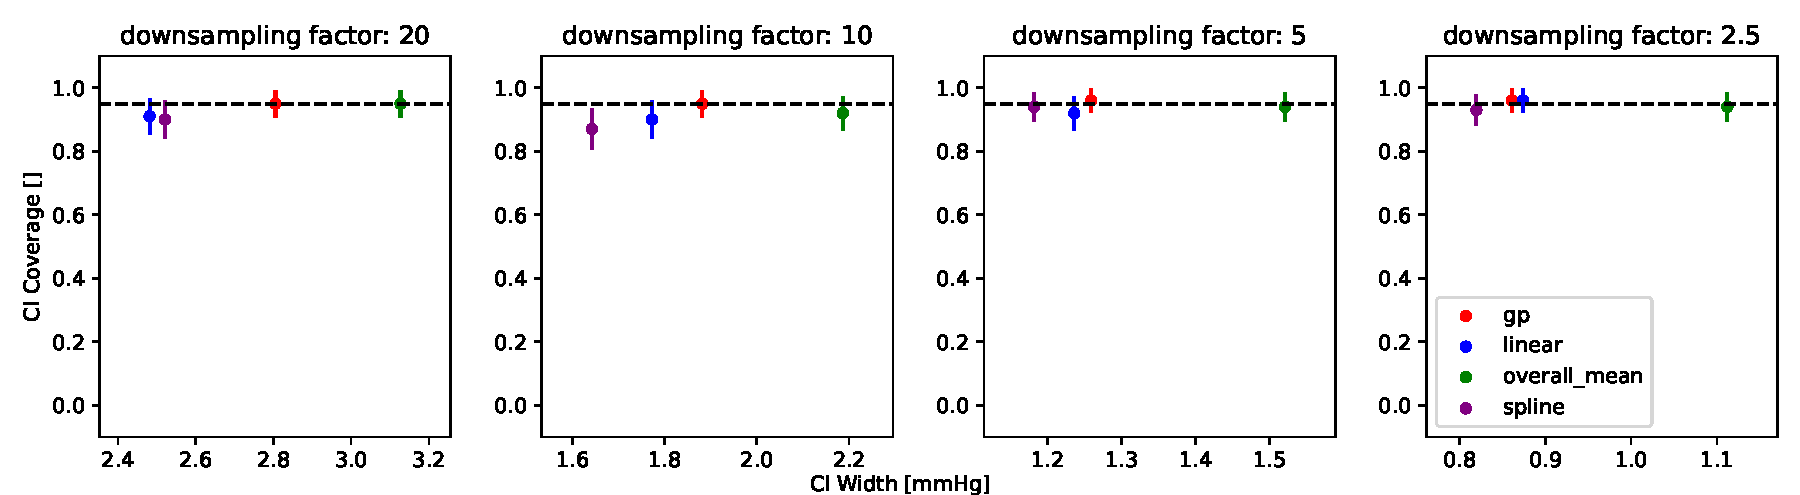
\includegraphics[width=\linewidth]{Pictures/final_experiment_hpdi/overall_mean_eval_sin_rbf_default}
    \caption{One-Week Mean - Uniform Downsampling}
    \label{fig:weekly-mean-uniform-sampling-performance}
\end{subfigure}

\bigskip

\begin{subfigure}{\textwidth}
    \centering
    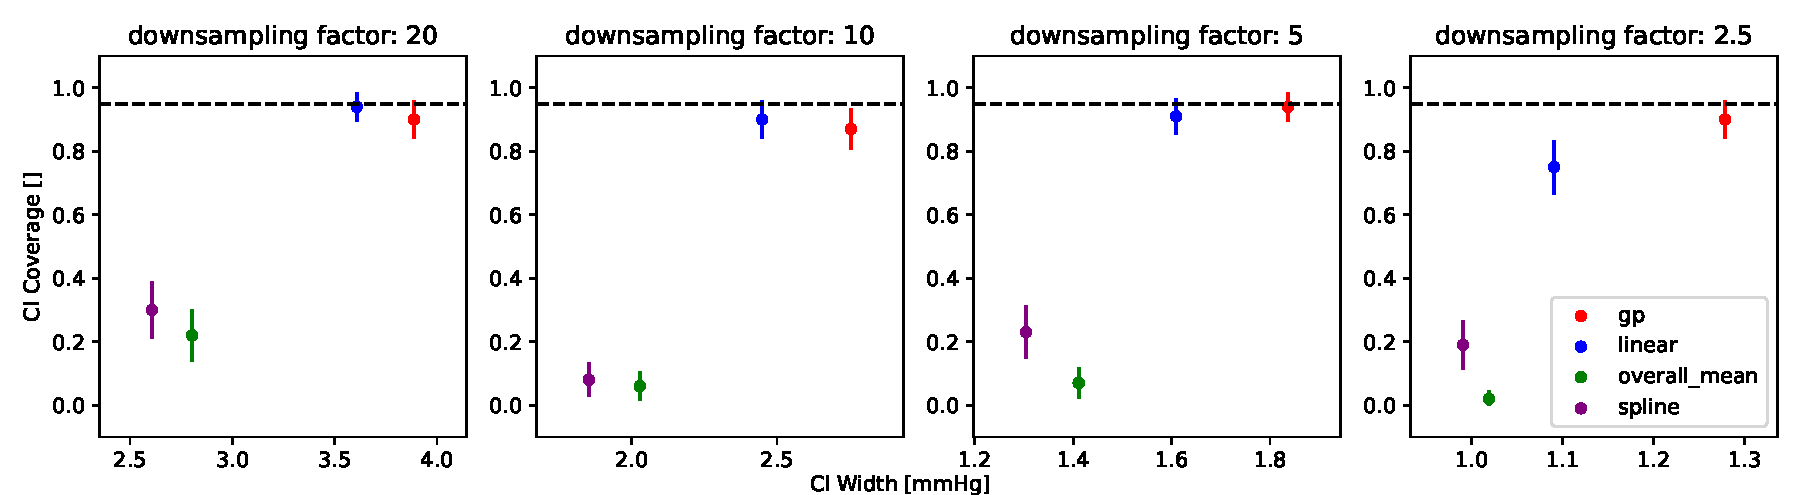
\includegraphics[width=\linewidth]{Pictures/final_experiment_hpdi/overall_mean_eval_sin_rbf_seasonal_default}
    \caption{One-Week Mean - Seasonal Downsampling}
    \label{fig:weekly-mean-seasonal-sampling-performance}
\end{subfigure}

\bigskip

\begin{subfigure}{\textwidth}
    \centering
    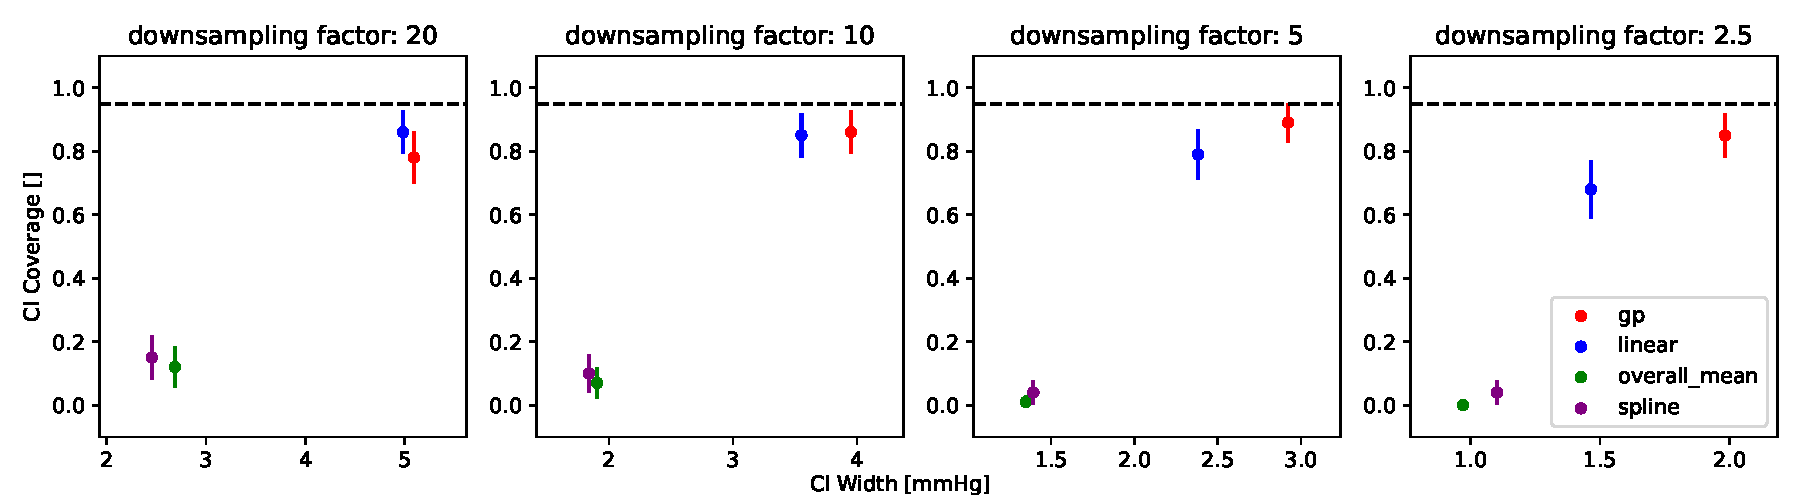
\includegraphics[width=\linewidth]{Pictures/final_experiment_hpdi/overall_mean_eval_sin_rbf_seasonal_extreme}
    \caption{One-Week Mean - Extreme Seasonal Downsampling}
    \label{fig:weekly-mean-extreme-seasonal-sampling-performance}
\end{subfigure}

\caption[One-Week Mean Performance]{The Performance of different methods to
estimate the one-week mean based on different downsampling patterns. The dashed horizontal line
indicates the target coverage of 95\% 
}
\label{fig:weekly-mean-performance}
\end{figure}



\subsection{One-Day and One-Hour Mean}

Figure \ref{fig:daily-mean-performance} and figure \ref{fig:daily-mean-performance}
show the Performance of different methods to
estimate the one-day and one-hour mean based on different downsampling patterns.

Best estimates are produced by GP regression for both the one-hour and one-day mean,
while the effect is more pronounced by the latter.
When not suffering too much from the estimation
instabiltiy described in the previous subsection,
spline interpolation does produce decent results.
In the face of uniform samplinng the one-day mean is aproxximated adequately also
by the naive ttr.
However, linear regression does not seem to be able to produce good estiamates
at this resolution.



\begin{figure}[!ht]
\centering
\begin{subfigure}{\textwidth}
    \centering
    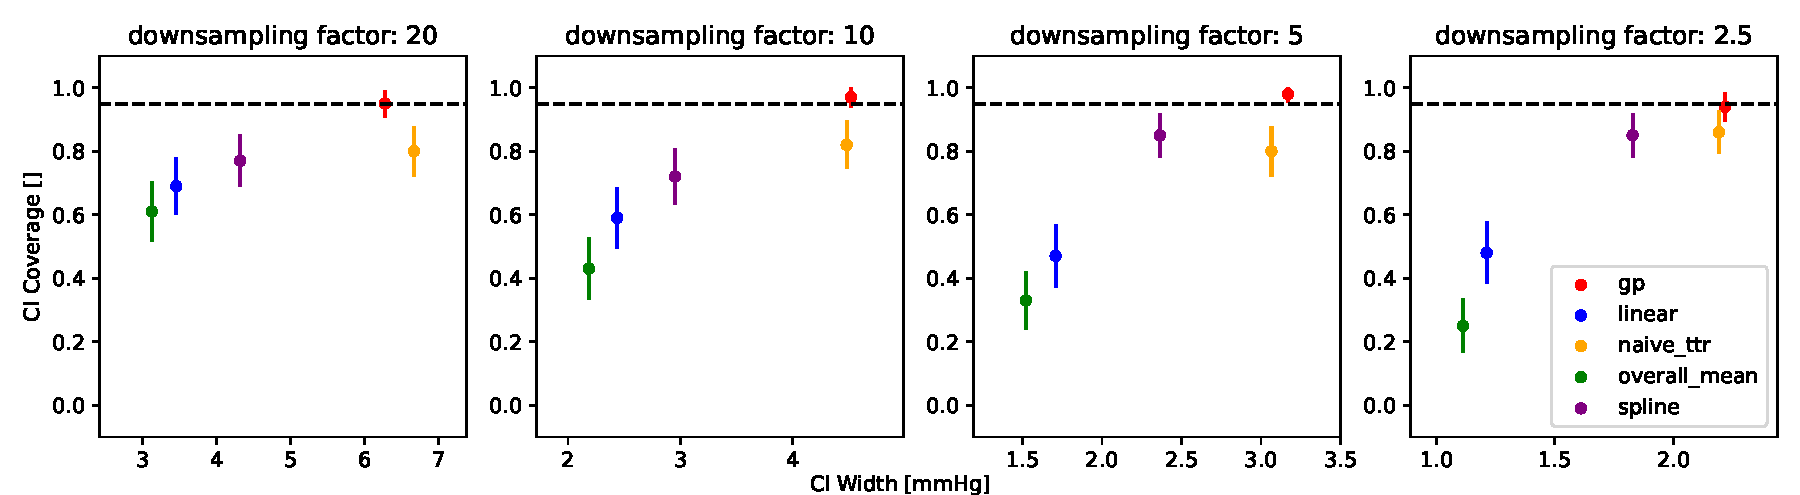
\includegraphics[width=\linewidth]{Pictures/final_experiment_hpdi/mean_24h_eval_sin_rbf_default}
    \caption{One-Day Mean Performance - Uniform Downsampling}
    \label{fig:daily-mean-uniform-sampling-performance}
\end{subfigure}

\bigskip

\begin{subfigure}{\textwidth}
    \centering
    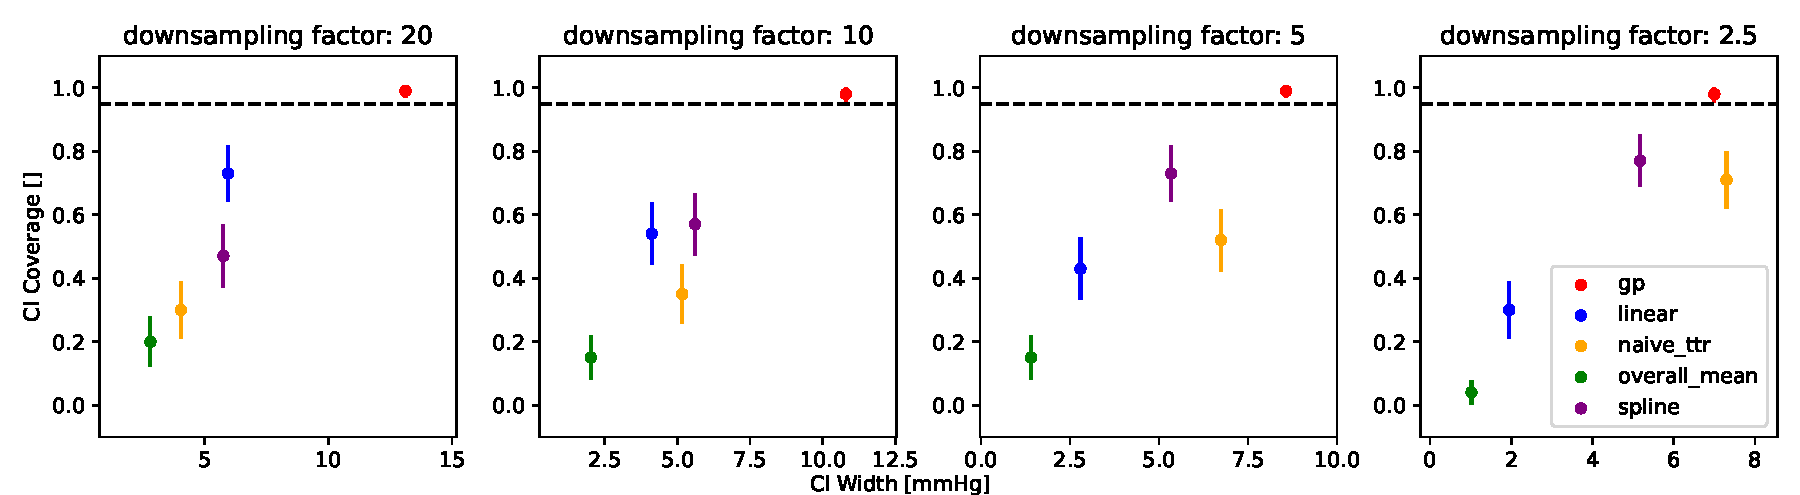
\includegraphics[width=\linewidth]{Pictures/final_experiment_hpdi/mean_1h_eval_sin_rbf_seasonal_default}
    \caption{One-Day Mean Performance - Seasonal Downsampling}
    \label{fig:daily-mean-seasonal-sampling-performance}
\end{subfigure}

\bigskip

\begin{subfigure}{\textwidth}
    \centering
    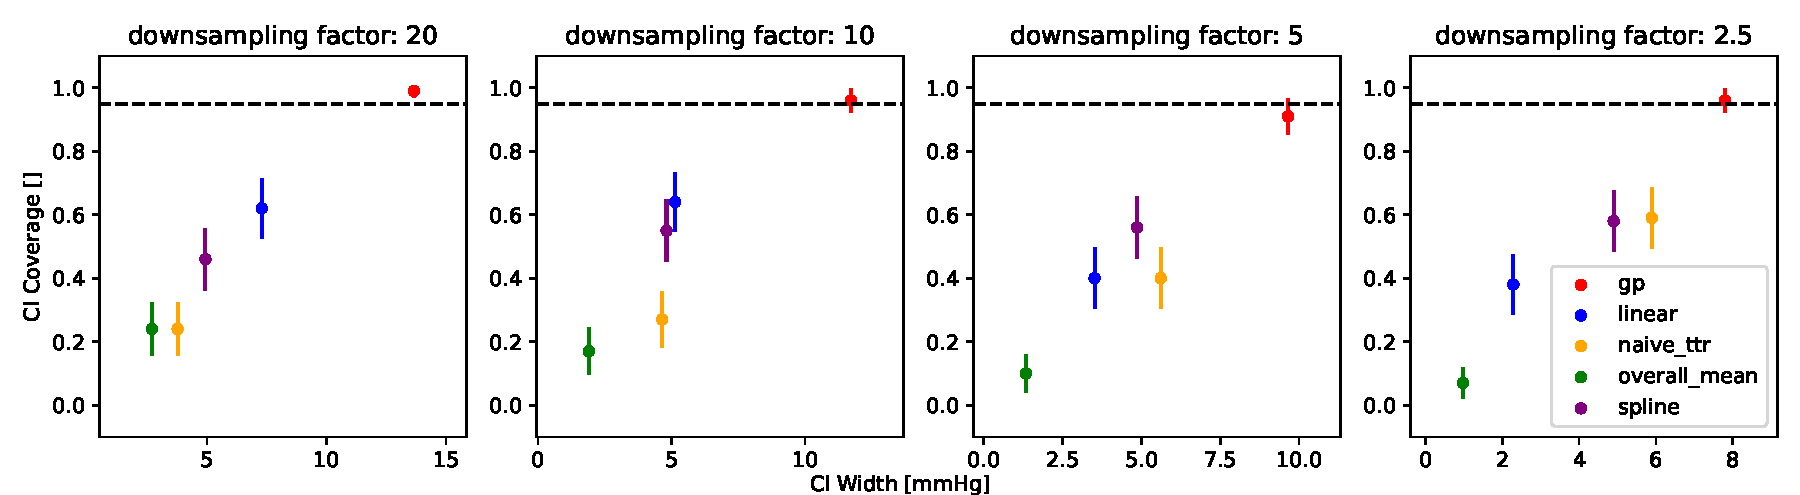
\includegraphics[width=\linewidth]{Pictures/final_experiment_hpdi/mean_1h_eval_sin_rbf_seasonal_extreme}
    \caption{One-Day Mean Performance - Extreme Seasonal Downsampling}
    \label{fig:daily-mean-extreme-seasonal-sampling-performance}
\end{subfigure}

\caption[One-Day Mean Performance]{The Performance of different methods to
estimate the one-day mean based on different downsampling patterns.
}
\label{fig:daily-mean-performance}
\end{figure}




\begin{figure}[!ht]
\centering
\begin{subfigure}{\textwidth}
    \centering
    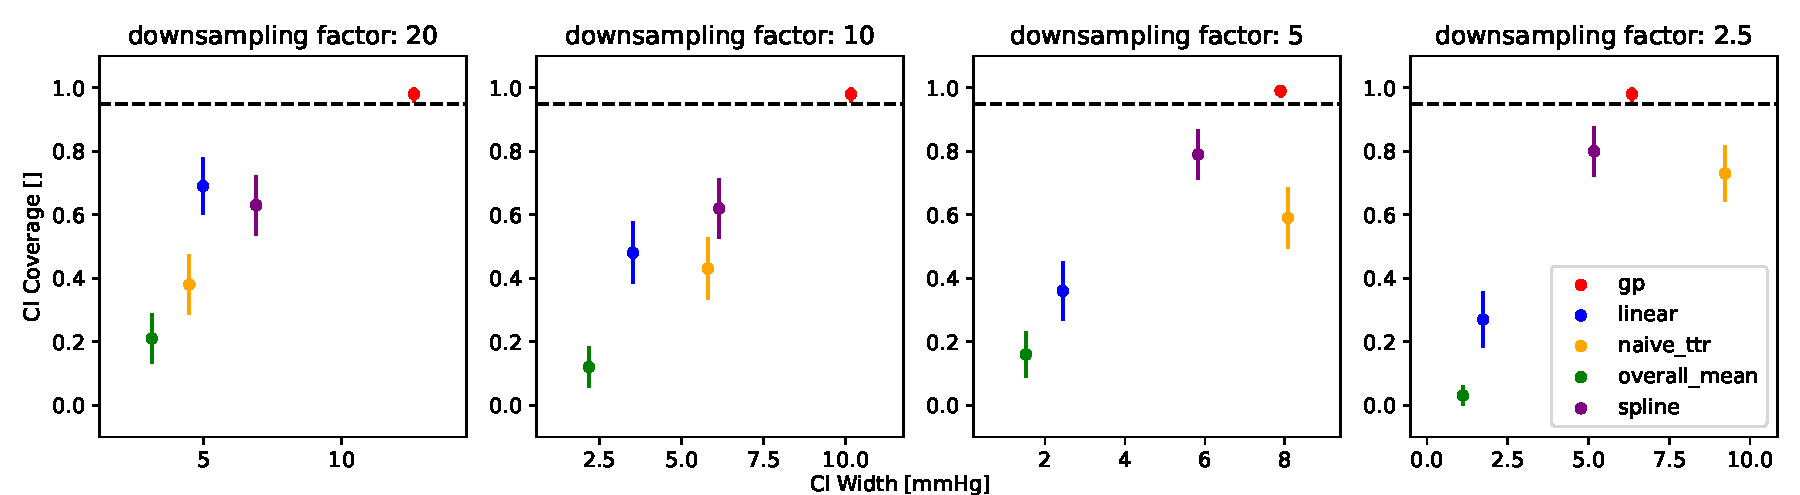
\includegraphics[width=\linewidth]{Pictures/final_experiment_hpdi/mean_1h_eval_sin_rbf_default}
    \caption{One-Hour Mean Performance - Uniform Downsampling}
    \label{fig:hourly-mean-uniform-sampling-performance}
\end{subfigure}

\bigskip

\begin{subfigure}{\textwidth}
    \centering
    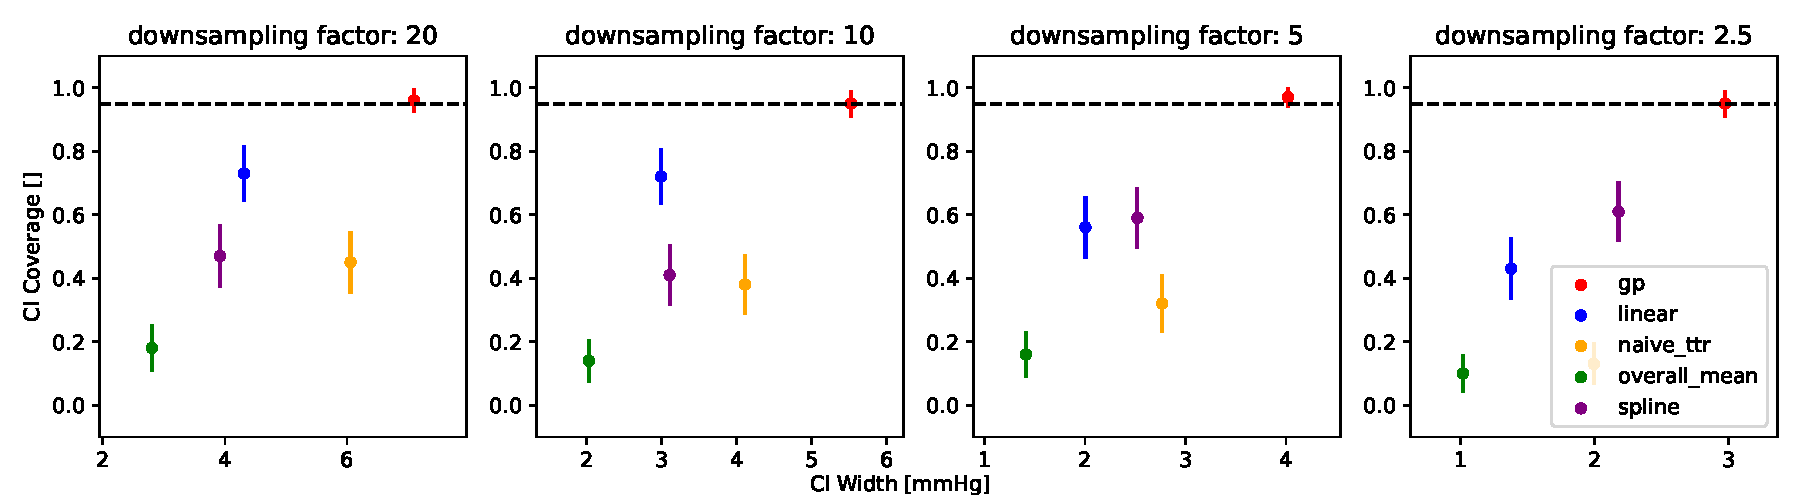
\includegraphics[width=\linewidth]{Pictures/final_experiment_hpdi/mean_24h_eval_sin_rbf_seasonal_default}
    \caption{One-Hour Mean Performance - Seasonal Downsampling}
    \label{fig:hourly-mean-seasonal-sampling-performance}
\end{subfigure}

\bigskip

\begin{subfigure}{\textwidth}
    \centering
    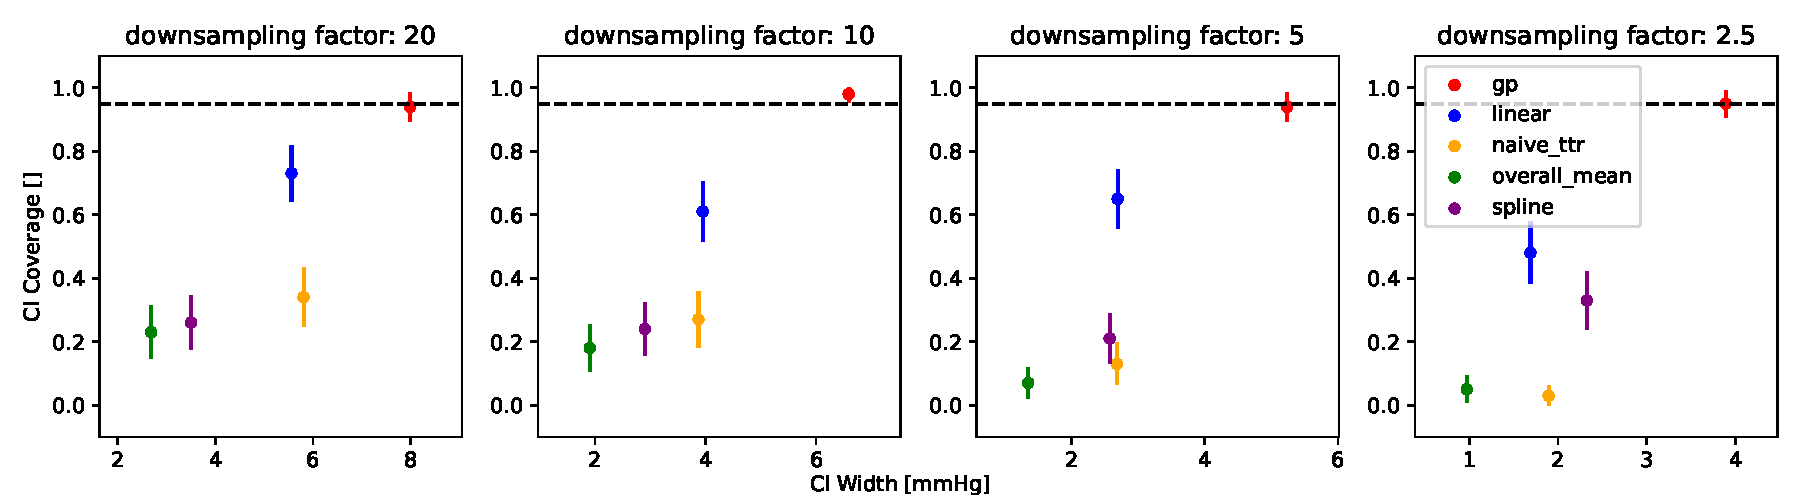
\includegraphics[width=\linewidth]{Pictures/final_experiment_hpdi/mean_24h_eval_sin_rbf_seasonal_extreme}
    \caption{One-Hour Mean Performance - Extreme Seasonal Downsampling}
    \label{fig:hourly-mean-extreme-seasonal-sampling-performance}
\end{subfigure}

\caption[One-Hour Mean Performance]{The Performance of different methods to
estimate the one-hour mean based on different downsampling patterns.
}
\label{fig:hourly-mean-performance}
\end{figure}


\subsection{Time in Target Range}

Figure \ref{fig:ttr-performance} shows the performance of different methods to
estimate time in target range (TTR) based on different downsampling patterns.
The only methods which sometimes reach the 95\% coverage target are
GP regression and smoothing spline interpolation, whereas GP regression produces
consistently lower CI width and does approach the target coverage with more
data.
Note that TTR does not care about the absolute values of the BP estimates
but does only check whether they are within the target range.
Since TTR is not affected by the extreme estimate values
occasionally produced by smoothing spline interpolation,
spline interpolation produces reasonable TTR estimates.
The current approach used to estimate TTR (naive\_ttr) performs very baldy.
This is since it does not estimate TTR through estimation of $f(x)$ but directly
works on the noisy measurements $Y(x)$. It will thus generally underestimate
TTR.


\begin{figure}[!ht]
\centering
\begin{subfigure}{\textwidth}
    \centering
    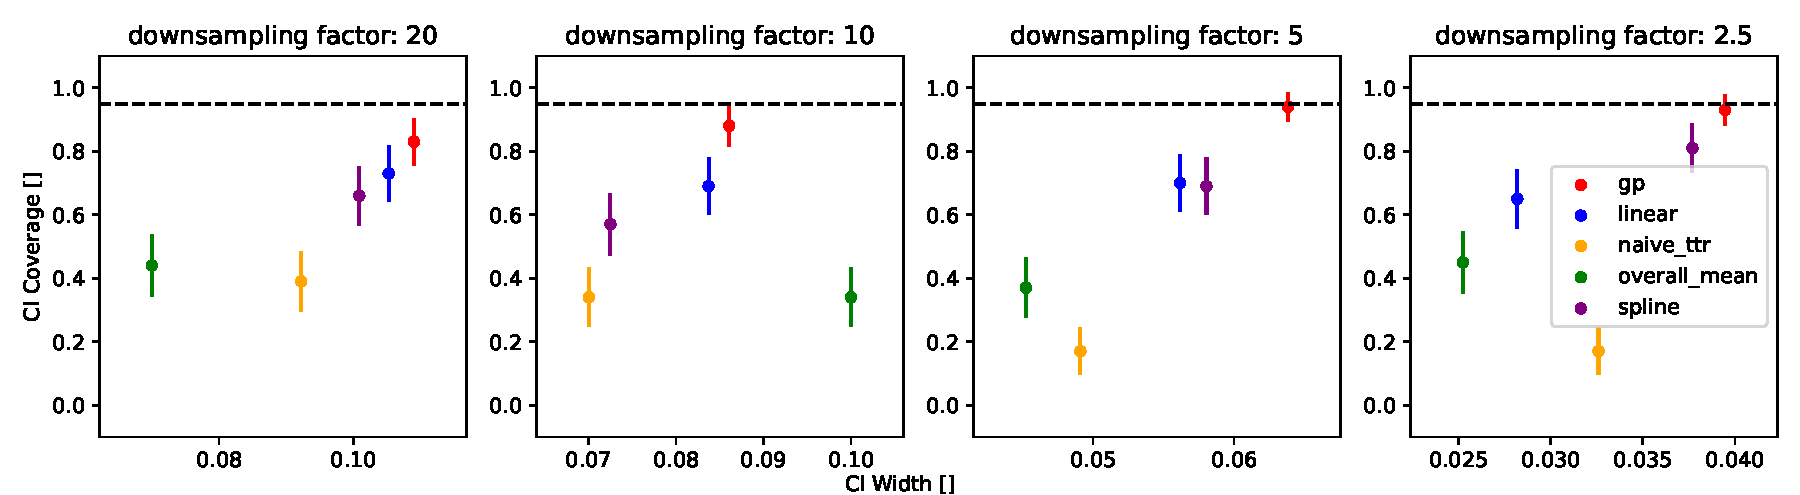
\includegraphics[width=\linewidth]{Pictures/final_experiment_hpdi/ttr_eval_sin_rbf_default}
    \caption{TTR Performance - Uniform Downsampling}
    \label{fig:ttr-uniform-sampling-performance}
\end{subfigure}

\bigskip

\begin{subfigure}{\textwidth}
    \centering
    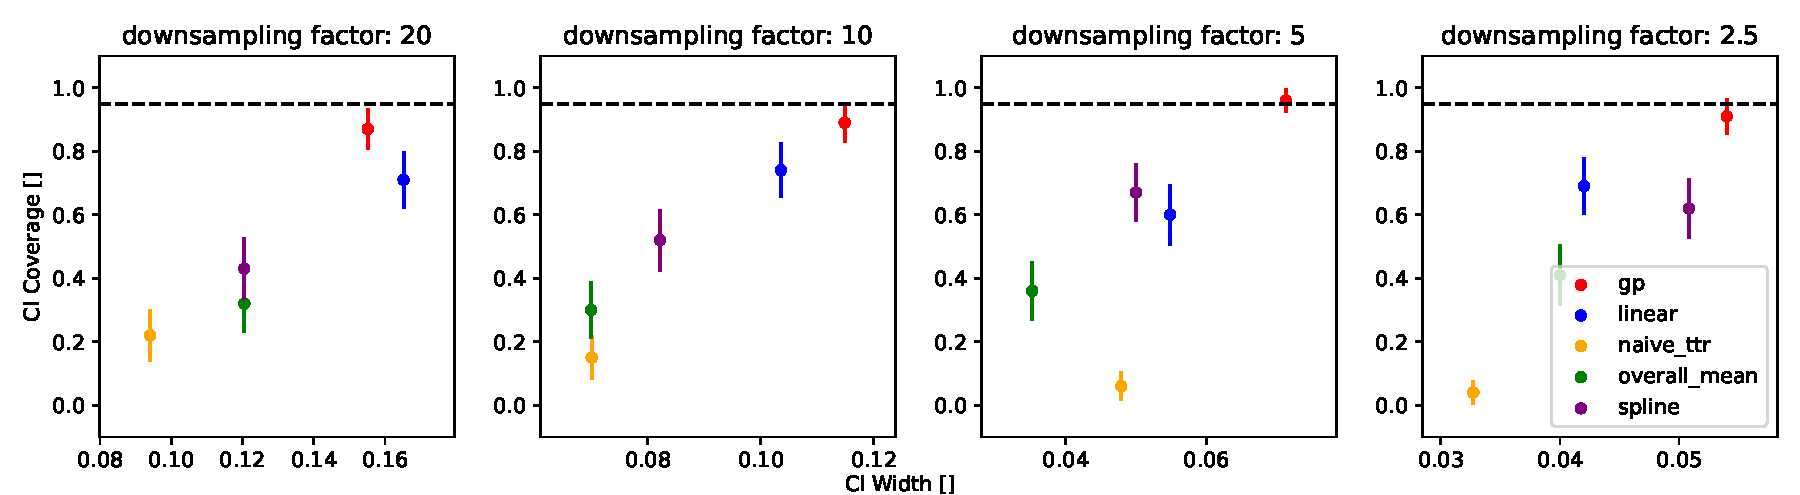
\includegraphics[width=\linewidth]{Pictures/final_experiment_hpdi/ttr_eval_sin_rbf_seasonal_default}
    \caption{TTR Performance - Seasonal Downsampling}
    \label{fig:ttr-seasonal-sampling-performance}
\end{subfigure}

\bigskip

\begin{subfigure}{\textwidth}
    \centering
    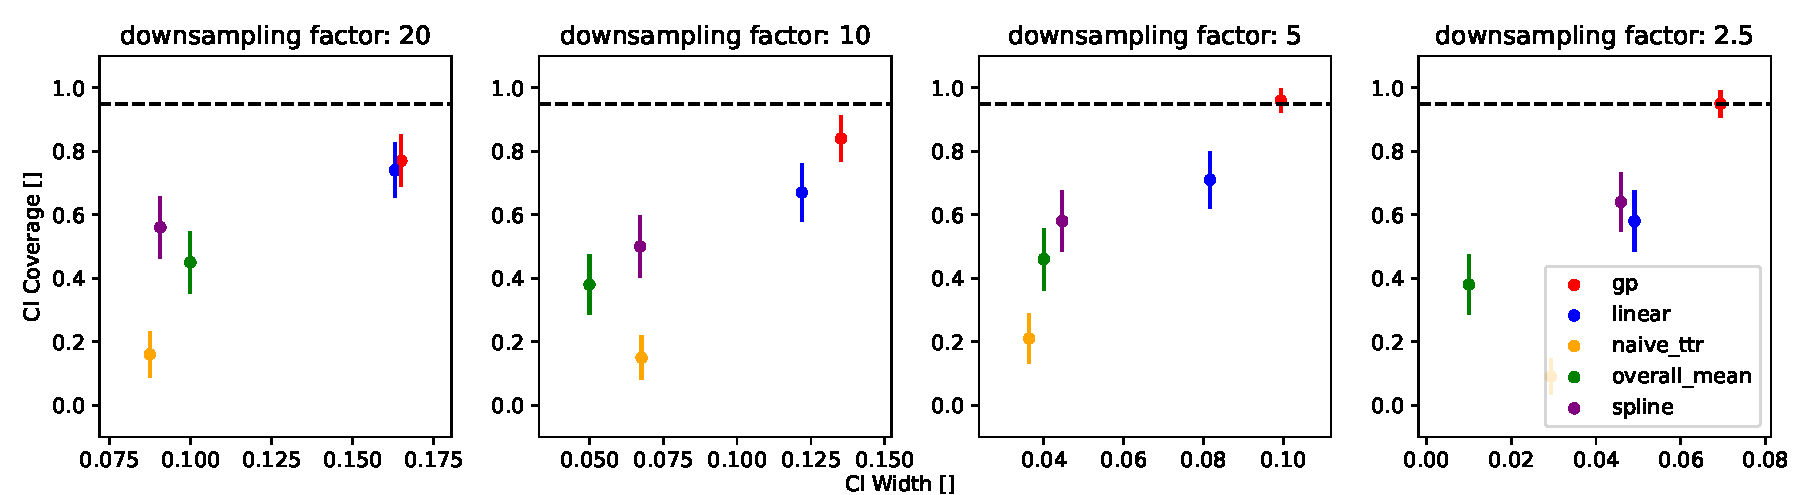
\includegraphics[width=\linewidth]{Pictures/final_experiment_hpdi/ttr_eval_sin_rbf_seasonal_extreme}
    \caption{TTR Performance - Extreme Seasonal Downsampling}
    \label{fig:ttr-extreme-seasonal-sampling-performance}
\end{subfigure}

\caption[TTR Performance]{The Performance of different methods to
estimate TTR based on different downsampling patterns.
}
\label{fig:ttr-performance}
\end{figure}





\section{Examples}


\subsection{Pronounced Cyclic Component}

\begin{figure}[!ht]
\centering
    \includegraphics[width=\linewidth]{Pictures/plots_final3/sin_rbf_default_0.2/09_11_09_05_45/plot_mean_decomposed_vertical}
\caption[Decomposed BP time sereis]{Left panel: Decomposition of the true BP time series $f(x)$. Right panel:
Decomposition of $\hat{f})x$ estimated using GP regression.}
\label{fig:ex1-gp-prediction}
\end{figure}

\begin{figure}[!ht]
\centering

\begin{subfigure}{.45\textwidth}
    \centering
    \includegraphics[width=\linewidth]{Pictures/plots_final3/sin_rbf_default_0.2/09_11_09_05_45/plot_posterior_spline}
  \caption[Spline]{Smoothing spline prediction}
  \label{fig:ex1-spline}
\end{subfigure}\hfill
\begin{subfigure}{.45\textwidth}
    \centering
    \includegraphics[width=\linewidth]{Pictures/plots_final3/sin_rbf_default_0.2/09_11_09_05_45/plot_posterior_linear}
  \caption[Linear Regression]{Linear regression prediction}
  \label{fig:ex1-linear}
\end{subfigure}
\begin{subfigure}{0.6\textwidth}
    \centering
    \includegraphics[width=\linewidth]{Pictures/plots_final3/sin_rbf_default_0.2/09_11_09_05_45/plot_posterior}
  \caption[GP Prediction]{GP Regression prediciton with predictive variance (gray area)}
  \label{fig:ex1-spline}
\end{subfigure}
\caption[True BP value prediction]{Prediction of true BP values $F_X$ (black) form measurments (red dots). The true BP values are shown
by the red dotted line. }
\label{fig:ex1}
\end{figure}


\subsection{Pronounced AR Component}

\begin{figure}[!ht]
\centering
    \includegraphics[width=\linewidth]{Pictures/plots_final3/sin_rbf_default_0.2/09_11_09_05_07/plot_mean_decomposed_vertical}
\caption[Decomposed BP time sereis]{Left panel: Decomposition of the true BP time series $f(x)$. Right panel:
Decomposition of $\hat{f})x$ estimated using GP regression.}
\label{fig:ex2-gp-prediction}
\end{figure}

\begin{figure}[!ht]
\centering

\begin{subfigure}{.45\textwidth}
    \centering
    \includegraphics[width=\linewidth]{Pictures/plots_final3/sin_rbf_default_0.2/09_11_09_08_20/plot_posterior_spline}
  \caption[Spline]{Smoothing spline prediction}
  \label{fig:ex2-spline}
\end{subfigure}\hfill
\begin{subfigure}{.45\textwidth}
    \centering
    \includegraphics[width=\linewidth]{Pictures/plots_final3/sin_rbf_default_0.2/09_11_09_08_20/plot_posterior_linear}
  \caption[Linear Regression]{Linear regression prediction}
  \label{fig:ex2-linear}
\end{subfigure}
\begin{subfigure}{0.6\textwidth}
    \centering
    \includegraphics[width=\linewidth]{Pictures/plots_final3/sin_rbf_default_0.2/09_11_09_08_20/plot_posterior}
  \caption[GP Prediction]{GP Regression prediciton with predictive variance (gray area)}
  \label{fig:ex2-gp}
\end{subfigure}
\caption[True BP value prediction]{Prediction of true BP values $F_X$ (black) form measurments (red dots). The true BP values are shown
by the red dotted line. }
\label{fig:ex2}
\end{figure}



\begin{figure}[!ht]
\centering
    \includegraphics[width=\linewidth]{Pictures/plots_final3/sin_rbf_default_0.2/09_11_09_05_07/plot_mean_decomposed_vertical}
\caption[Decomposed BP time sereis]{Left panel: Decomposition of the true BP time series $f(x)$. Right panel:
Decomposition of $\hat{f})x$ estimated using GP regression.}
\label{fig:ex2-gp-prediction}
\end{figure}

\begin{figure}[!ht]
\centering
\begin{subfigure}{.45\textwidth}
    \centering
    \includegraphics[width=\linewidth]{Pictures/plots_final3/sin_rbf_default_0.2/09_11_09_08_20/plot_posterior_spline}
  \caption[Spline]{Smoothing spline prediction}
  \label{fig:ex2-spline}
\end{subfigure}\hfill
\begin{subfigure}{.45\textwidth}
    \centering
    \includegraphics[width=\linewidth]{Pictures/plots_final3/sin_rbf_default_0.2/09_11_09_08_20/plot_posterior_linear}
  \caption[Linear Regression]{Linear regression prediction}
  \label{fig:ex2-linear}
\end{subfigure}
\begin{subfigure}{0.6\textwidth}
    \centering
    \includegraphics[width=\linewidth]{Pictures/plots_final3/sin_rbf_default_0.2/09_11_09_08_20/plot_posterior}
  \caption[GP Prediction]{GP Regression prediciton with predictive variance (gray area)}
  \label{fig:ex2-gp}
\end{subfigure}
\caption[True BP value prediction]{Prediction of true BP values $F_X$ (black) form measurments (red dots). The true BP values are shown
by the red dotted line. }
\label{fig:ex2}
\end{figure}



\subsection{Smoothing Spline Failure}
Figure \ref{fig:ex-spline-failure} illustrates how spline regression
produces  very
large confidence interval for high downsampling factors.
Boostrapping in these conditions leads to very instable BP estimates,
which is shown in figure \ref{subfig: ex-spline-failure-bootstrap}.
The estimated BP values $F_X$, from one boostrap sample, comprises very extreme BP values, which will
lead to underestimation of the one-week mean.

\begin{figure}[!ht]
\centering
\begin{subfigure}{.5\textwidth}
    \centering
    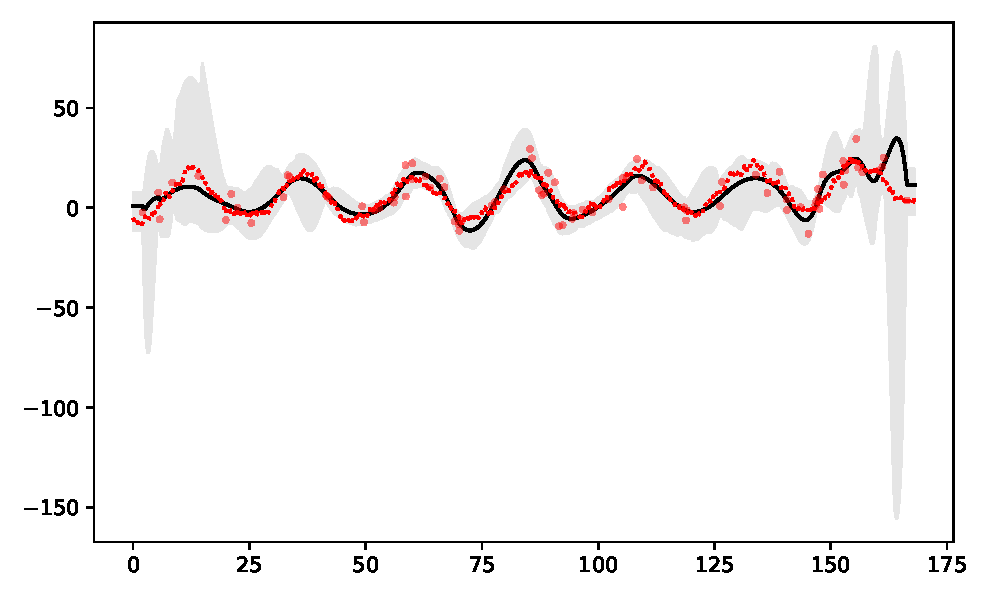
\includegraphics[width=\linewidth]{Pictures/spline_extreme/plot_posterior_confint_spline}
    \caption{Smoothing Spline PB estimates (black line), which is the mean over 100 botstrap samples.
    The true BP values red dotted line) are shown with training samples (red dots)}
\end{subfigure}\hfill
\begin{subfigure}{.42\textwidth}
    \centering
    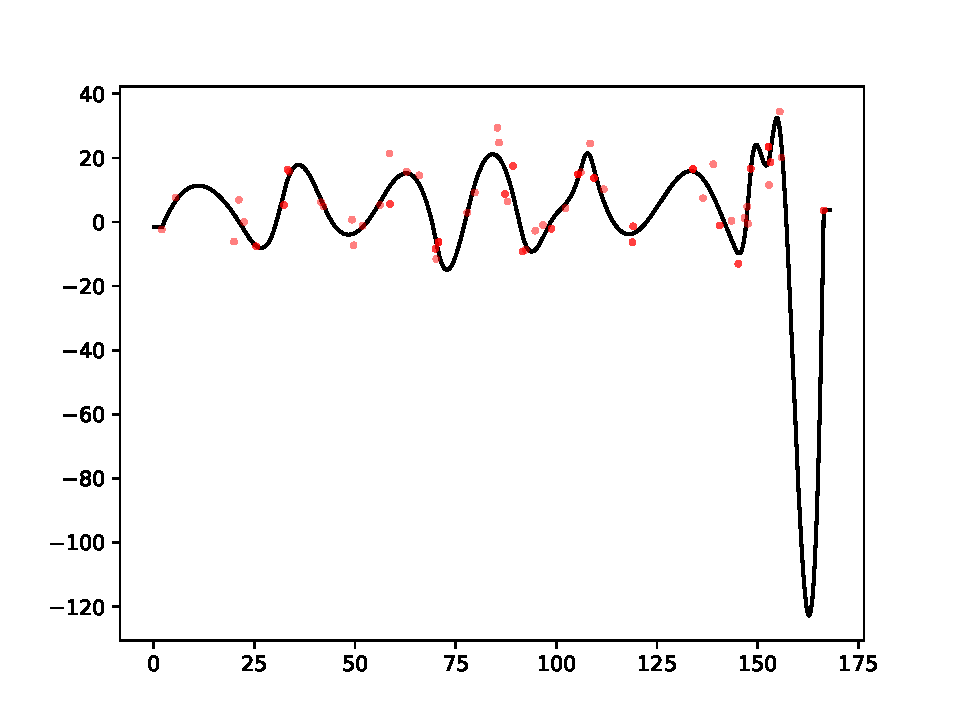
\includegraphics[width=\linewidth]{Pictures/spline_extreme/plot_pred_bootstrap_spline_reg_v2_70}
  \caption[Estimate Single Bootstrap Sample]{
      BP value estimates (black line) based on samples of one bootstrap iteration (red dots). This would
  lead to an extreme underestimation of the one-week mean.}
    \label{subfig: ex-spline-failure-bootstrap}
\end{subfigure}
\caption[Smoothing Spline Failure]{
    Smoothing spline giving extreme local predictions of the true BP values $f(x)$
    for a downsampling factor of 2.
    The huge drop produced at the end of the one week window
    leads to huge confidence intervals}
\label{fig:ex-spline-failure}
\end{figure}






%\begin{example}
%
%\begin{figure}[!ht]
%\centering
%\includegraphics[width=\linewidth]{Pictures/plots_final2/sin_rbf_default_0.2/09_11_07_49_51/plot_posterior}
%\caption[GP Prediction]{Predictive mean of $F_{X}$ (blackline) with
%predictive variance (grey area) based on observations (red dots) }
%\label{fig:ex1-gp-prediction}
%\end{figure}
%
%\begin{figure}[!ht]
%\centering
%\includegraphics[width=\linewidth]{Pictures/plots_final2/sin_rbf_default_0.2/09_11_07_49_51/plot_mean_decomposed}
%\caption[Mean Decomposed Predicted vs True]{Each figure shows one sample $F_X$ drawn from the true GP (red dashed line) with noisy observations
%  (red dots) sampled at a frequency of 0.5/hour}
%\label{fig:ex1-gp-mean-decomposed}
%\end{figure}
%
%
%\begin{figure}[!ht]
%\centering
%\begin{subfigure}{.45\textwidth}
%    \centering
%    \includegraphics[width=\linewidth]{Pictures/plots_final2/sin_rbf_default_0.2/09_11_07_49_51/plot_posterior_spline}
%  \caption[Spline]{The sample $F_X$ shown to the right, decomposed in to the contribution of the Periodic kernel (orange),
%      Matérn kernel (blue), RBF kernel (green).}
%  \label{fig:ex1-spline}
%\end{subfigure}\hfill
%\begin{subfigure}{.45\textwidth}
%    \centering
%    \includegraphics[width=\linewidth]{Pictures/plots_final2/sin_rbf_default_0.2/09_11_07_49_51/plot_posterior_linear}
%  \caption[Linear Regression]{Each figure shows one sample $F_X$ drawn from the true GP (red dashed line) with noisy observations
%      (red dots) sampled at a frequency of 0.5/hour}
%  \label{fig:ex1-linear}
%\end{subfigure}
%\caption[Baseline Methods]{Baseline Methods Example Prediction}
%\label{fig:ex1}
%\end{figure}
%



%\end{example}









